% DOC SETTINGS ===================================
\documentclass{article}
\usepackage[utf8]{inputenc}
\usepackage{fancyhdr}
\pagestyle{fancy}
\usepackage{geometry}
 \geometry{
 a4paper,
 total={170mm,257mm},
 left=20mm,
 top=25mm,
 }
\fancyheadoffset{0mm}
\lhead{ECE4540 Lab0}
\rhead{Kavin Thirukonda 2021}
\usepackage{steinmetz}
\usepackage{listings}
\usepackage{circuitikz}
\usepackage{wrapfig}
\usepackage{mathtools}  
\usepackage[font=small]{caption}
\mathtoolsset{showonlyrefs} 
\cfoot{}
% DOC SETTINGS ===================================
\begin{document}
\section*{Part 1}
\begin{enumerate}
    \item Please briefly describe what the following processing steps do. Do NOT just copy and paste from external resources. Use your own words.
    \begin{enumerate}
        \item Oxidation: Introducing oxygen to a portion of silicon where a silicon dioxide layer is desired, which causes the chemical reaction between the silicon and oxygen to for said silicon dioxide layer.
        \item Ion implantation: implanting ions of higher or lower valence in the silicon to manipulate the electrical characteristics 
        \item Diffusion: a property that represents the concentration of the chemicals in silicon electronics.
        \item Deposition: A process that describes a subset of methods used to layer on the required needs of a transistor such as the conductive and not conductive portions.
        \item Photo-lithography: A CAD etching process to create indents where needed for sometimes cosmetics and other time or more practical reasons
        \item Etching: Similar to photo lithography but its on a larger scale for anything that is too durable to complete the photo lithography process on.
    \end{enumerate}
    \item In figure 1.38 (c) in the textbook (reproduced below), there is an extra n+ region on the right, inside of the n-well. It is usually called a “well tap”. There is one similar p+ “substrate tap” on the left. These highly doped implant regions have low resistance.What is the purpose of these taps?How should we connect them(e.g. connecting to VDD, GND, IN,OUT or left floating)? Briefly explain your answer.
    \begin{center}
        \boxed{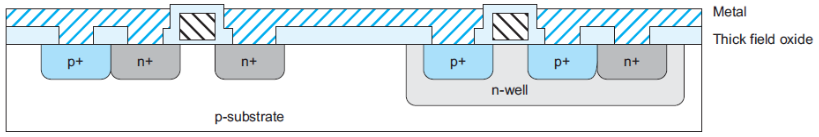
\includegraphics[width = .75\textwidth]{138c.png}}
    \end{center}
    \begin{center}
        The well taps are positive and negative well taps are connected to VDD and GND to prevent drift which would cause a latchup issue. When MOSFETS were first implemented this was not a design feature but as it evolved designers figured out that they could use well taps to avoid latchup.
    \end{center}
\end{enumerate}
\newpage
\section*{Part 2}
\subsection*{Section A:First Order Model}
\begin{itemize}
    \item T = 85C
    \item $\epsilon = 8.85\cdot10^{-14} F/cm$
    \item $t_{ox}$ = 1.14 (nm)
    \item $\mu_n$ = $670 (cm^2/V \cdot s)$, $\mu_p$ = $160 (cm^2/V \cdot s)$
    \item $V_{TN} = 0.410V,V_{TP} = -0.384V$
\end{itemize}
\begin{enumerate}
    \item Plot the Ids-Vds curve for \textbf{NMOS} for the following list of configurations:
    \begin{itemize}
        \item L = 50nm, W = 200nm
        \item \vline Vds \vline : range 0 - 1.1V
        \item \vline Vgs \vline : 0V, 0.2V, 0.4V, 0.6V, 0.8V, 1.1V
    \end{itemize}
    \begin{center}
        \boxed{\includegraphics[width = .55\textwidth]{idsvsvds.png}}
    \end{center}
    \begin{center}
        Dotted line represents the divide between the linear region and the saturation region.
    \end{center}
    \item Plot the Ids-Vgs curve for \textbf{PMOS} for the following list of configurations:
    \begin{itemize}
        \item L = 50nm, W = 200nm
        \item \vline Vgs \vline : range 0 - 1.1V
        \item \vline Vds \vline : 0V, 0.2V, 0.4V, 0.6V, 0.8V, 1.1V
    \end{itemize}
    \begin{center}
        \boxed{\includegraphics[width = .55\textwidth]{idsvsvds2.png}}
    \end{center}
    \begin{center}
        Dotted line represents the divide between the linear region and the saturation region.
    \end{center}
\end{enumerate}
\newpage
\subsection*{Section B:Free PDK 45nm Model}
\begin{enumerate}
    \item Redo the NMOS and PMOS plots from section A but in cadence.
    \begin{center}
        \boxed{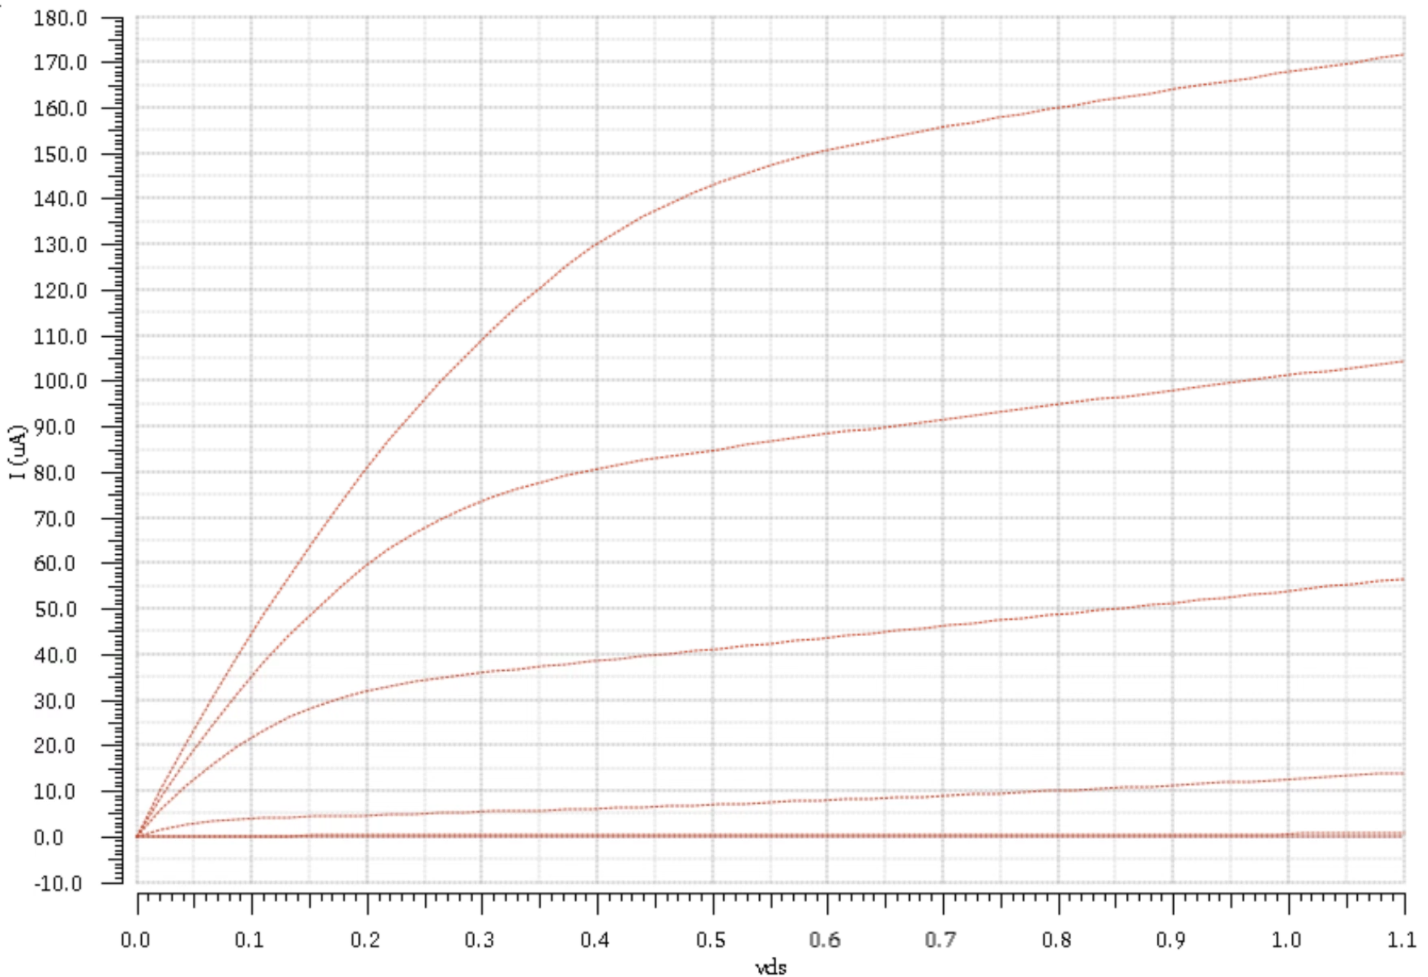
\includegraphics[width = .75\textwidth]{cadencenmos.png}}
    \end{center}
    \begin{center}
        \boxed{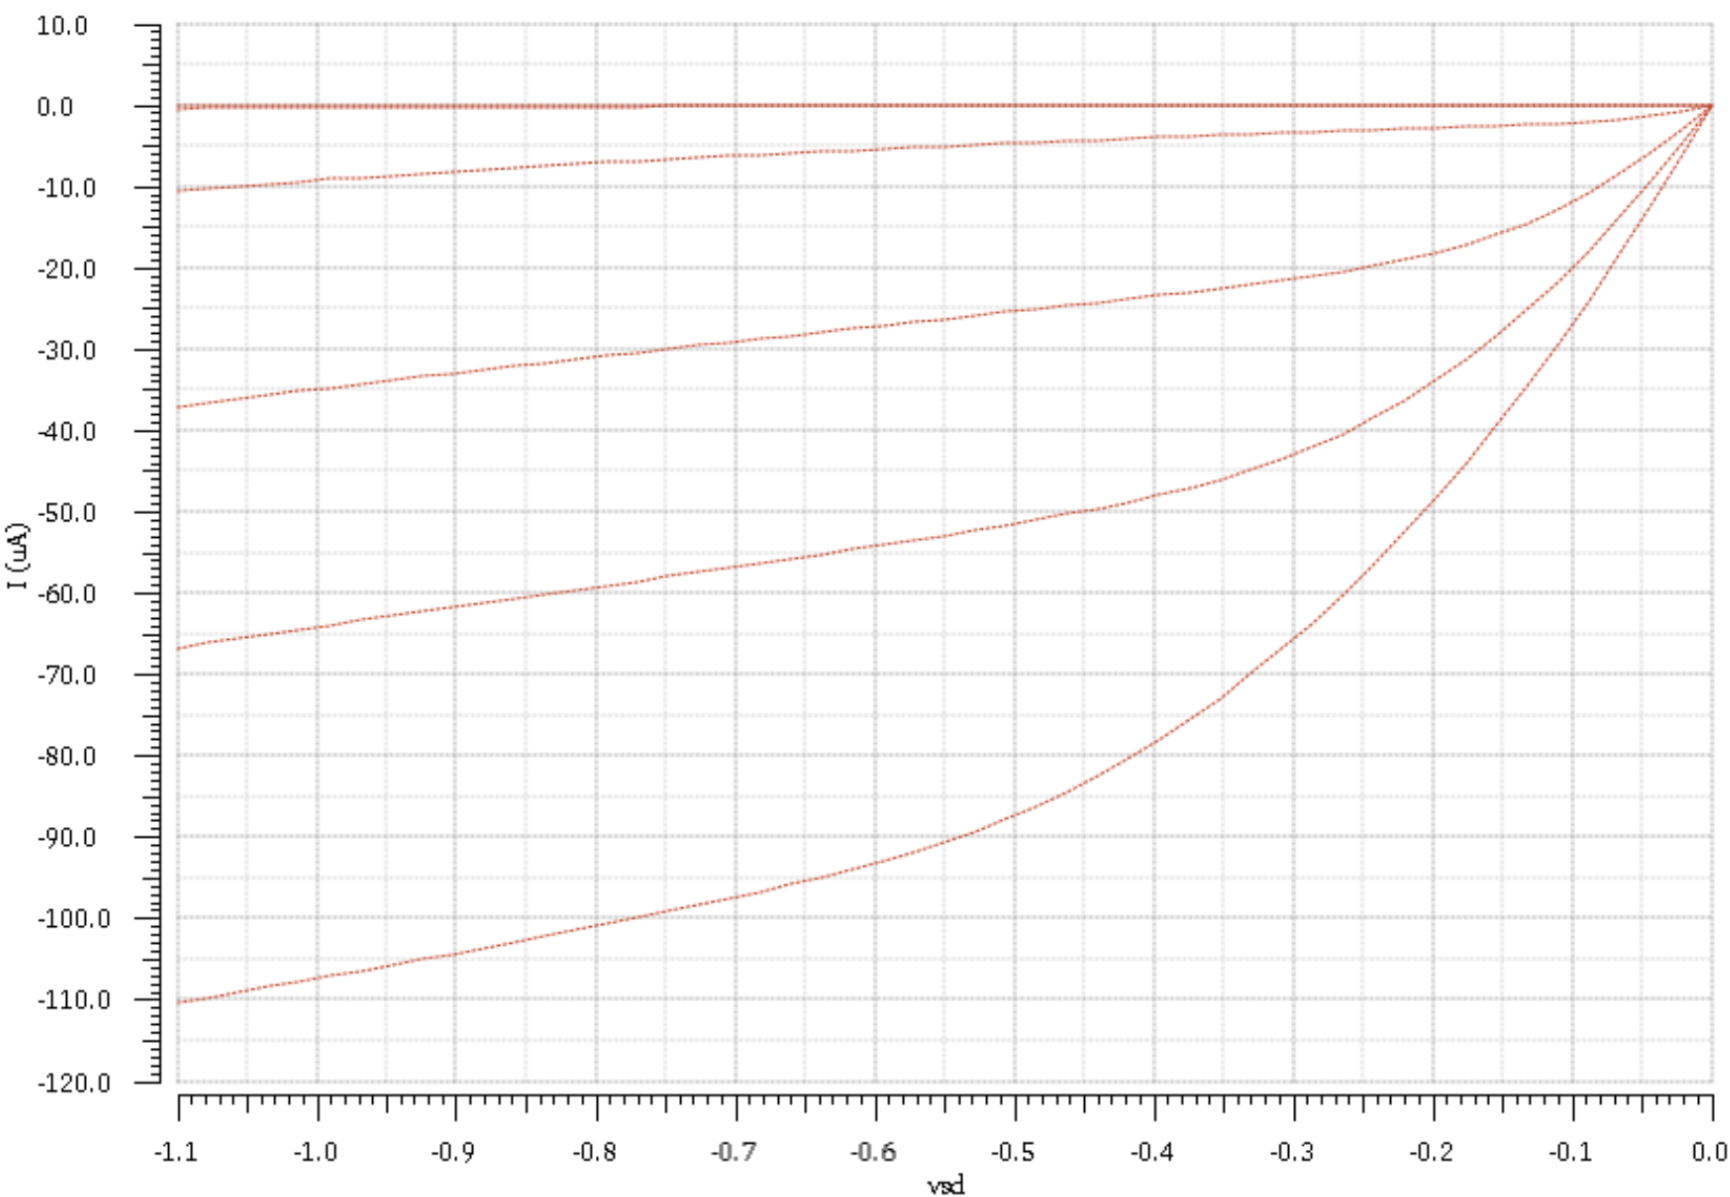
\includegraphics[width = .75\textwidth]{cadencepmos.png}}
    \end{center}
    \begin{center}
        The plots are mostly similar except the saturation region isnt as flat as the first order model would have you believe, its much more linear just not to the degree that it is in the actual linear region. another important thing to note is that, even though on the first order model it say that anything under the threshold voltage should be zero on the cadence model there is still some amount of current that gets passed on which did not occur on the first order model.
    \end{center}
    \newpage
    \item Redo part the two plots in part B with the following three $V_{sb}$ voltages: -0.5V, 0V, and 0.5V.Do you see any differences between the curves.
    \begin{center}
        \boxed{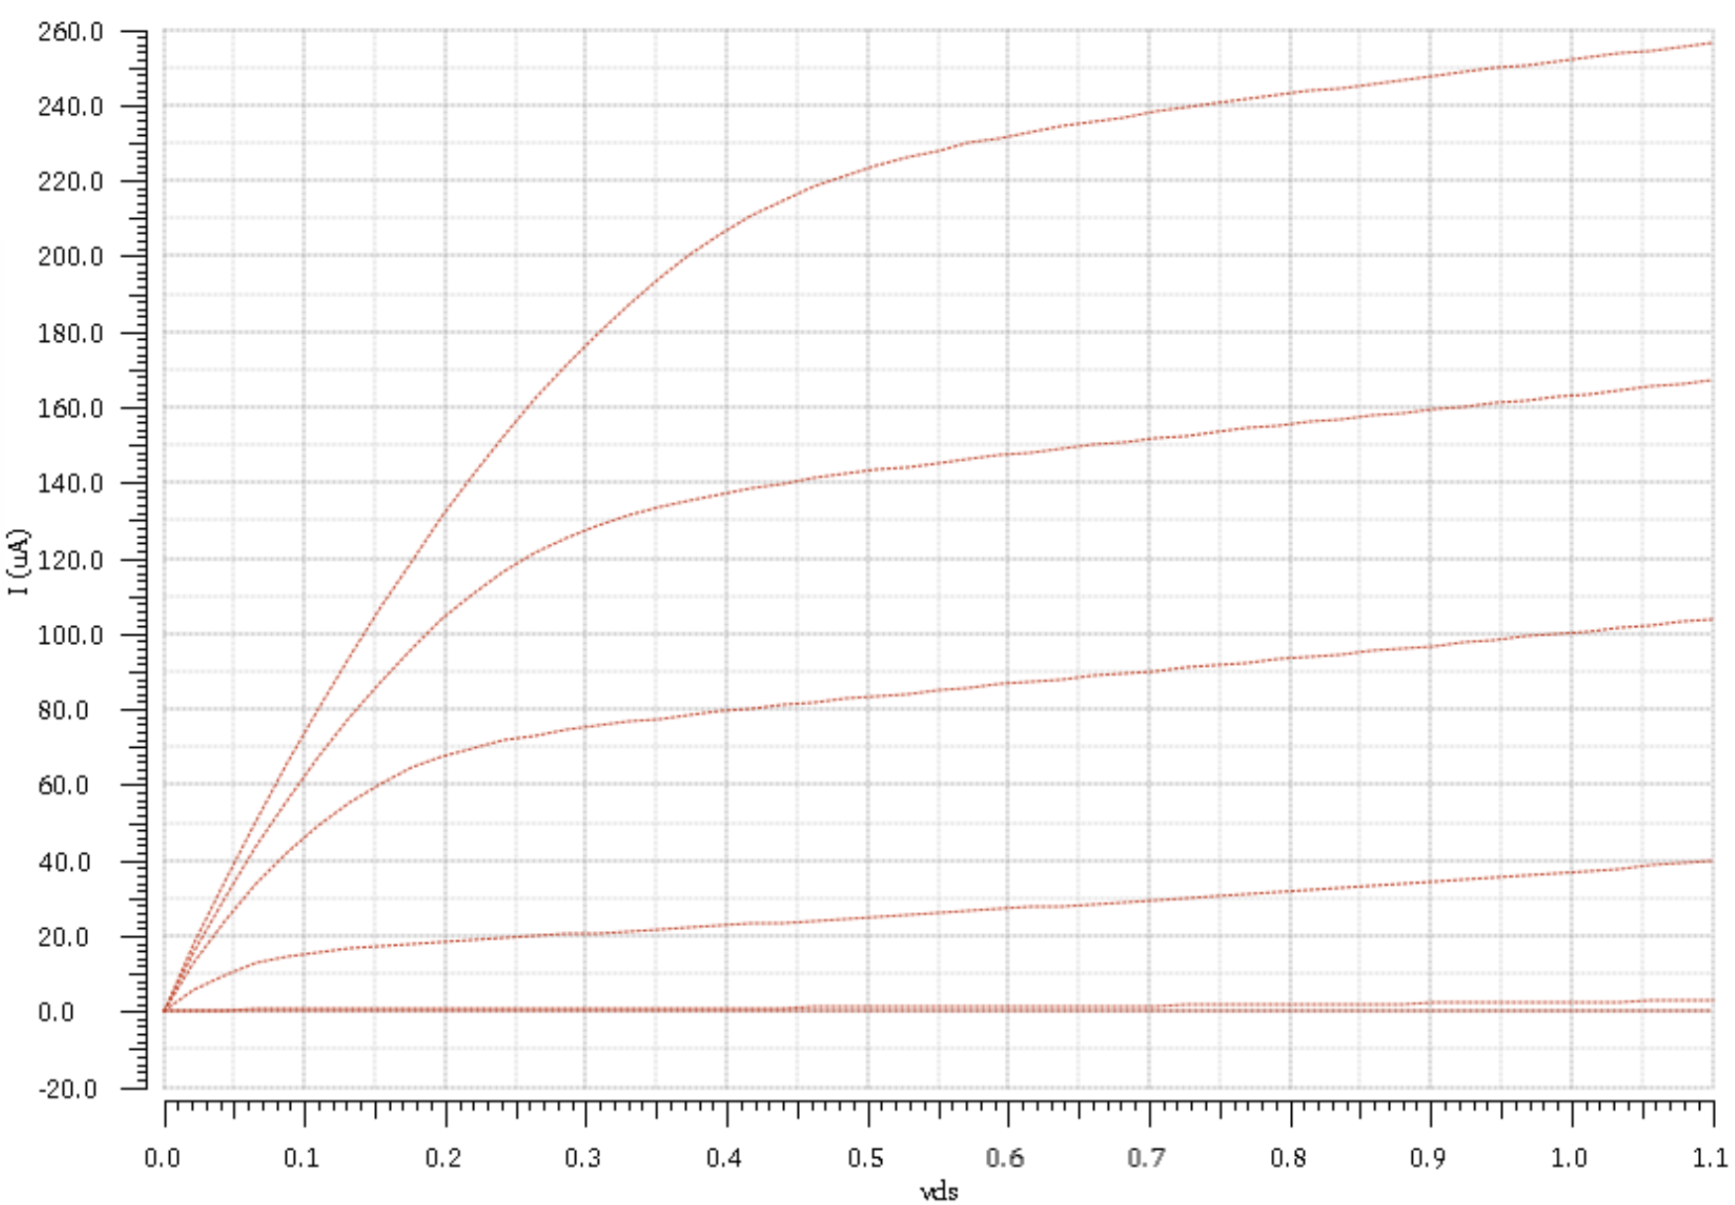
\includegraphics[width = .5\textwidth]{nmos5.png}}
        
        NMOS: $V_B = 0.5V$
    \end{center}
    \begin{center}
        \boxed{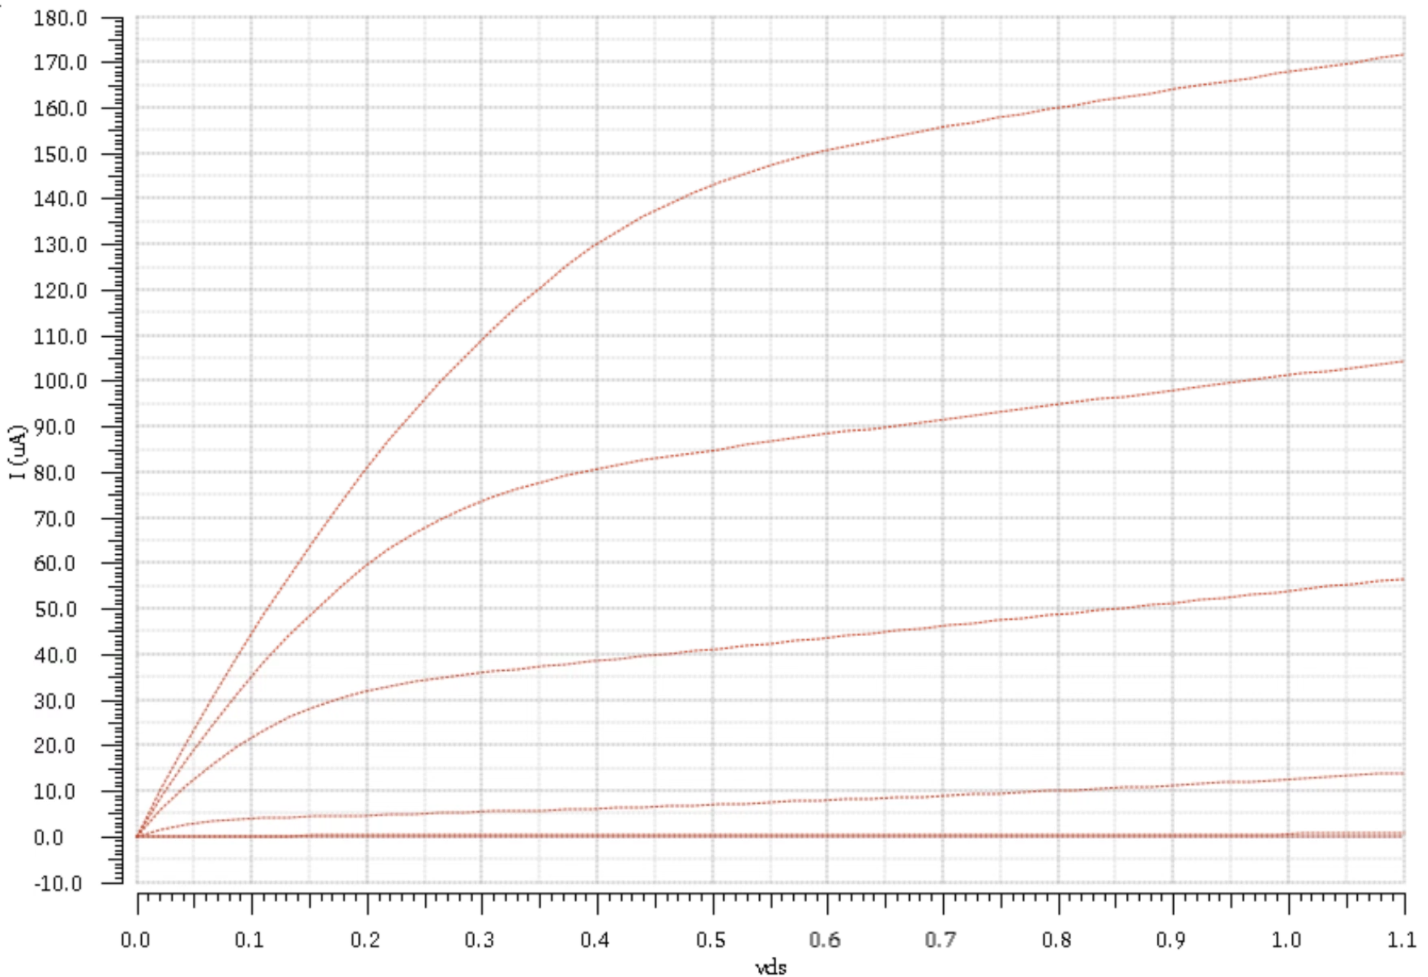
\includegraphics[width = .5\textwidth]{cadencenmos.png}}
        
        NMOS: $V_B = 0V$
    \end{center}
    \begin{center}
        \boxed{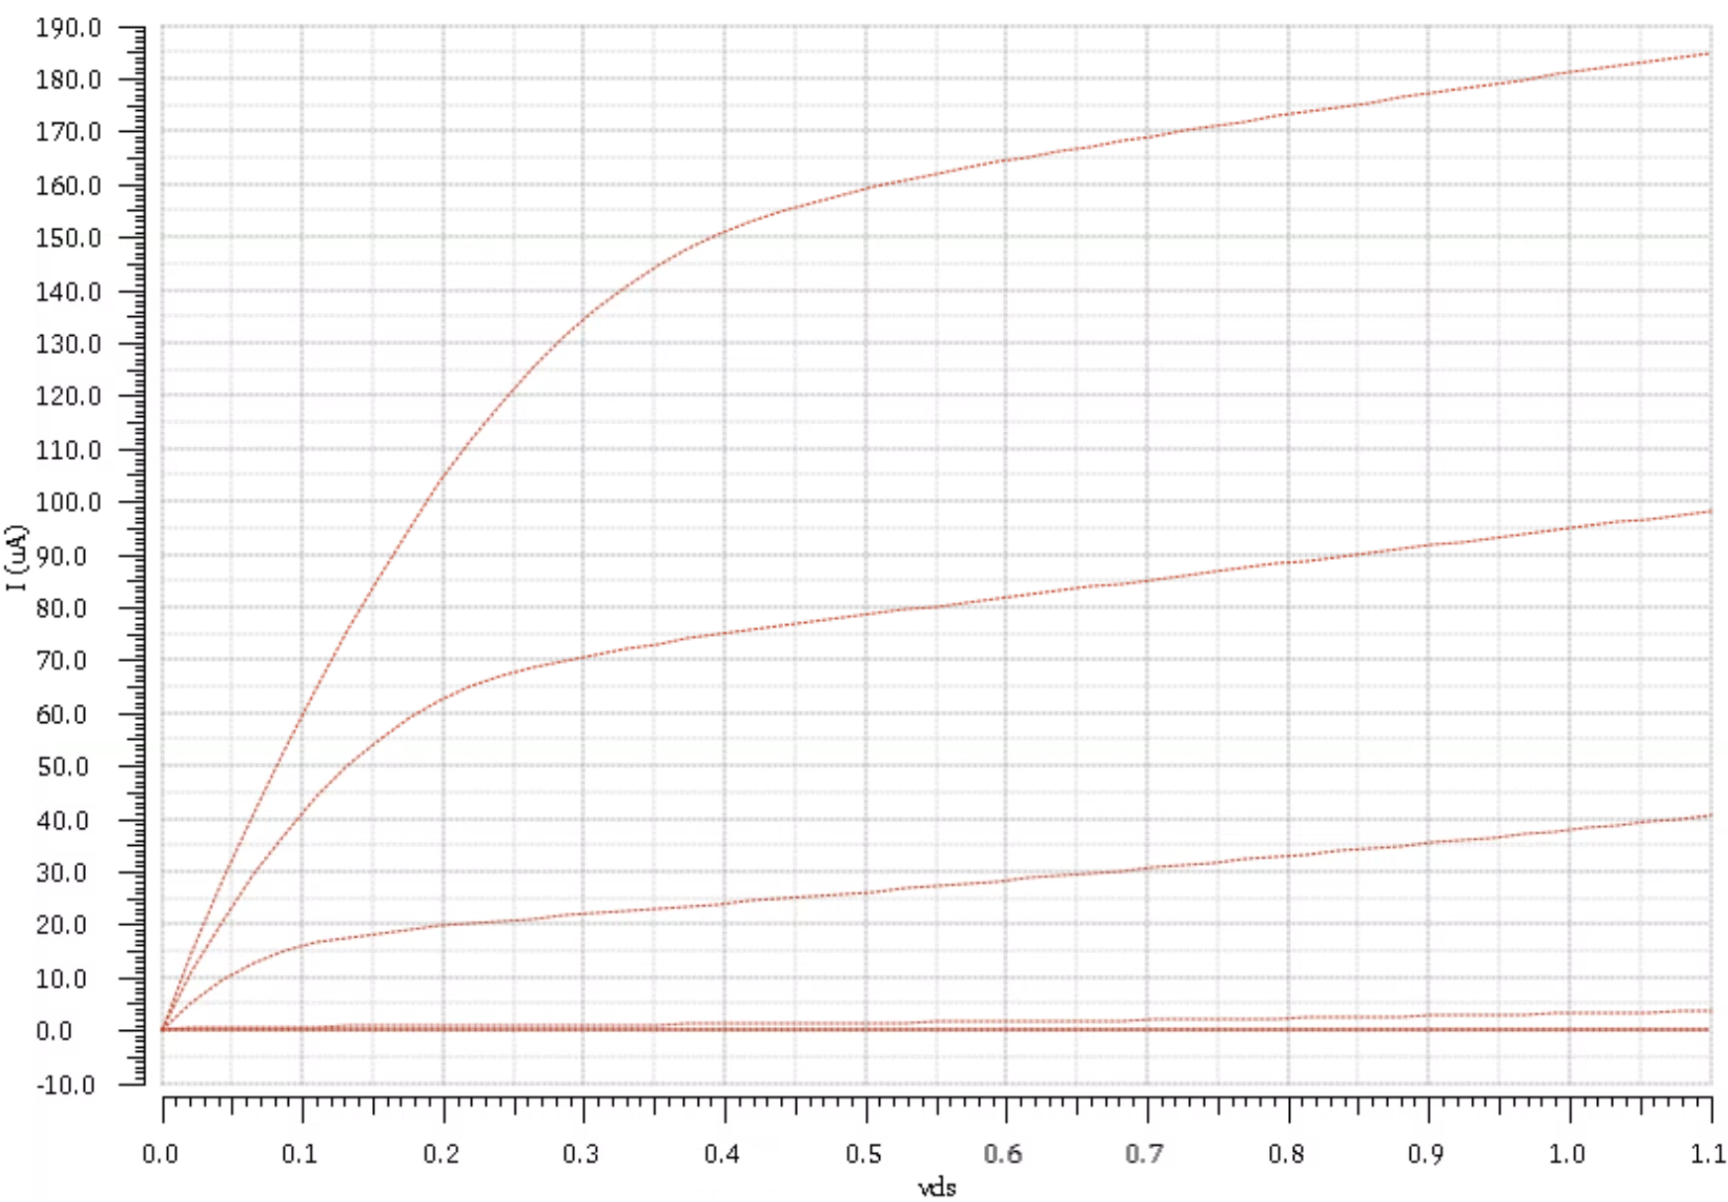
\includegraphics[width = .5\textwidth]{nmos-5.png}}
        
        NMOS: $V_B = -0.5V$
    \end{center}
    \begin{center}
        \boxed{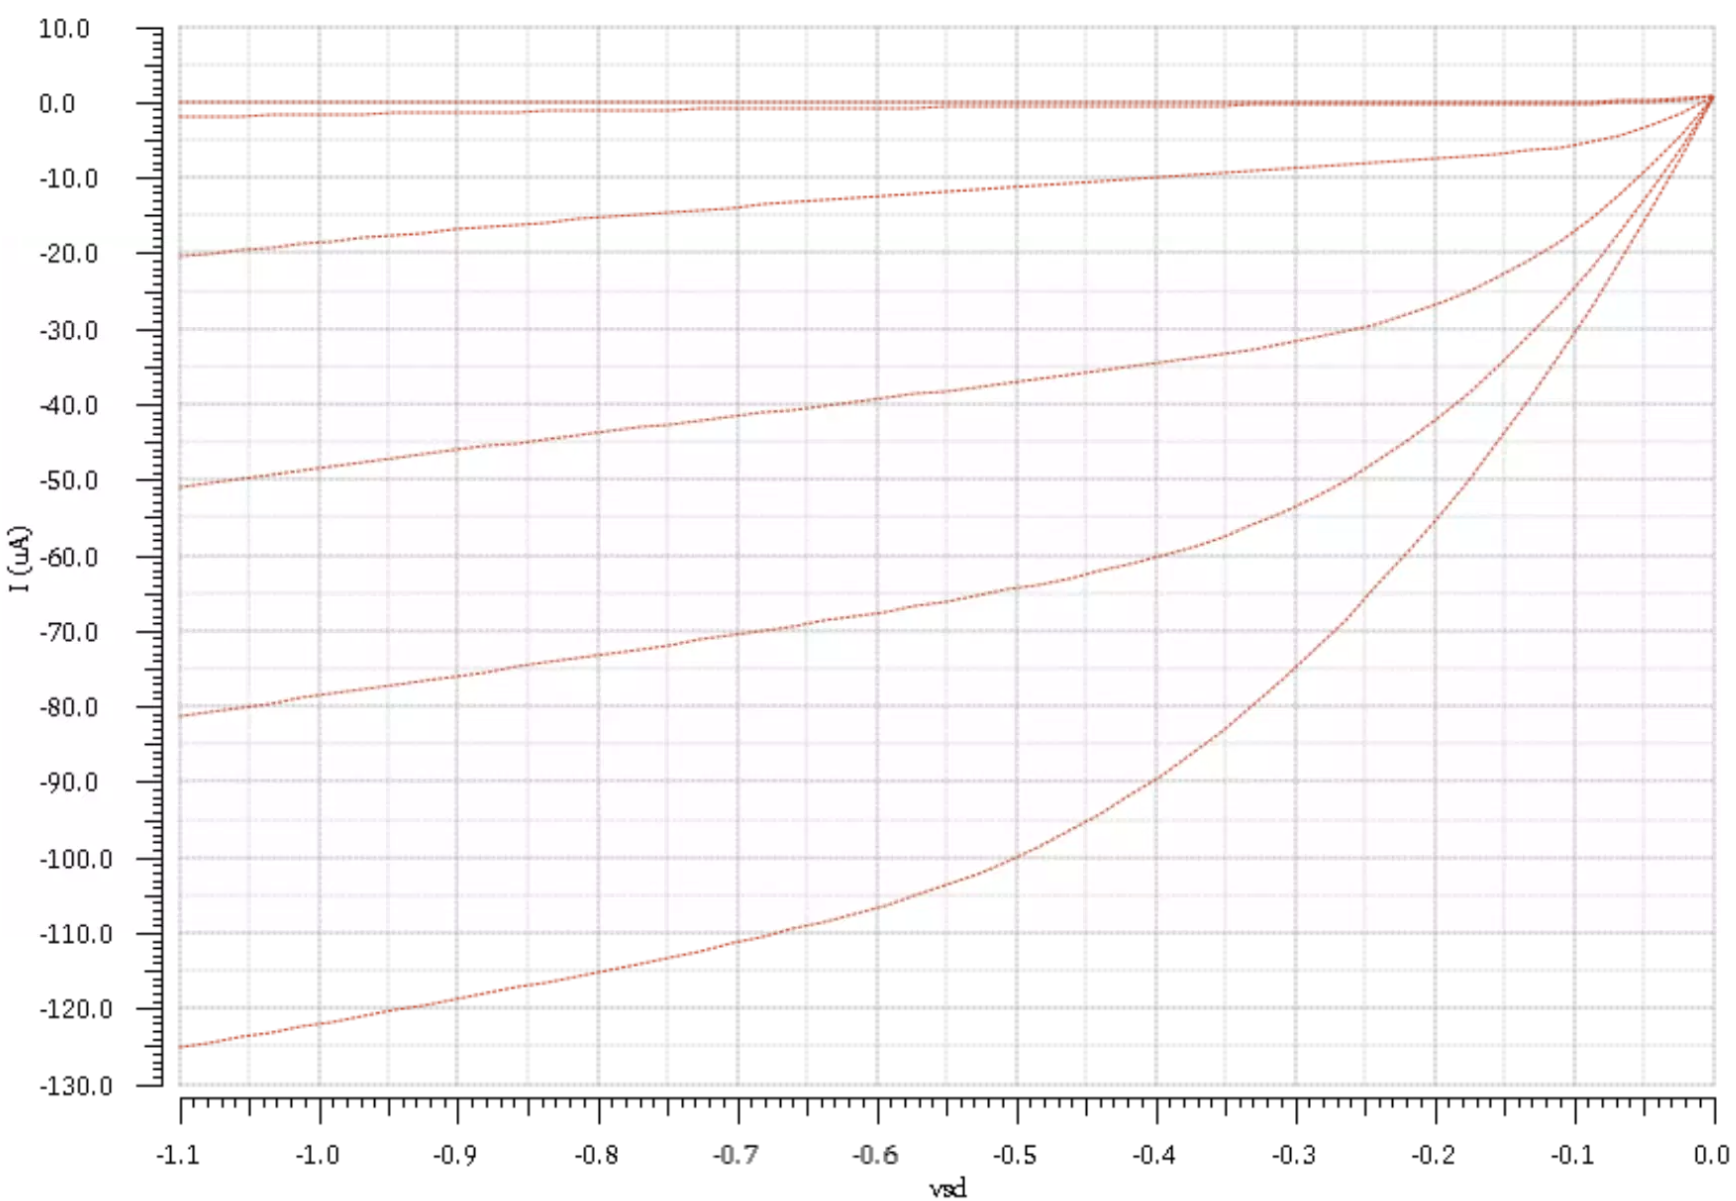
\includegraphics[width = .5\textwidth]{pmos5.png}}
        
        PMOS: $V_B = 0.5V$
    \end{center}
    \begin{center}
        \boxed{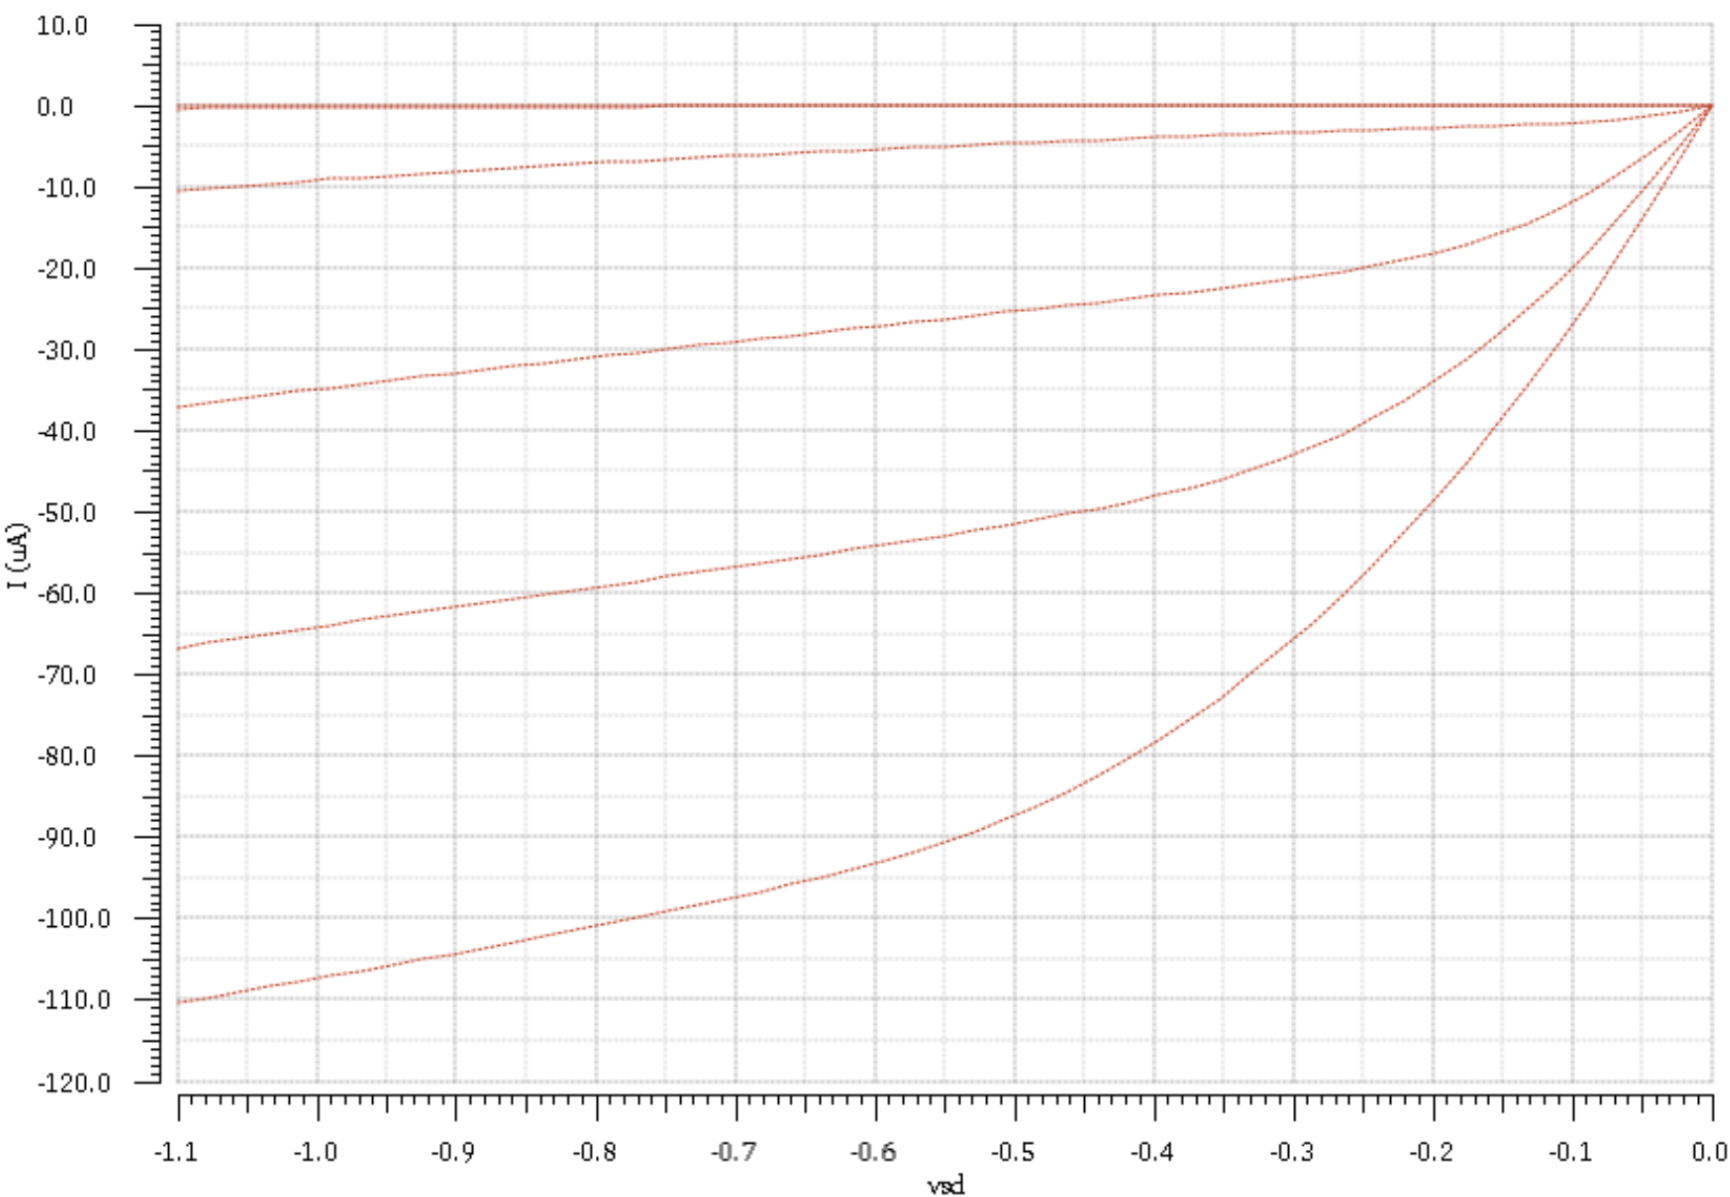
\includegraphics[width = .5\textwidth]{cadencepmos.png}}
        
        PMOS: $V_B = 0V$
    \end{center}
    \begin{center}
        \boxed{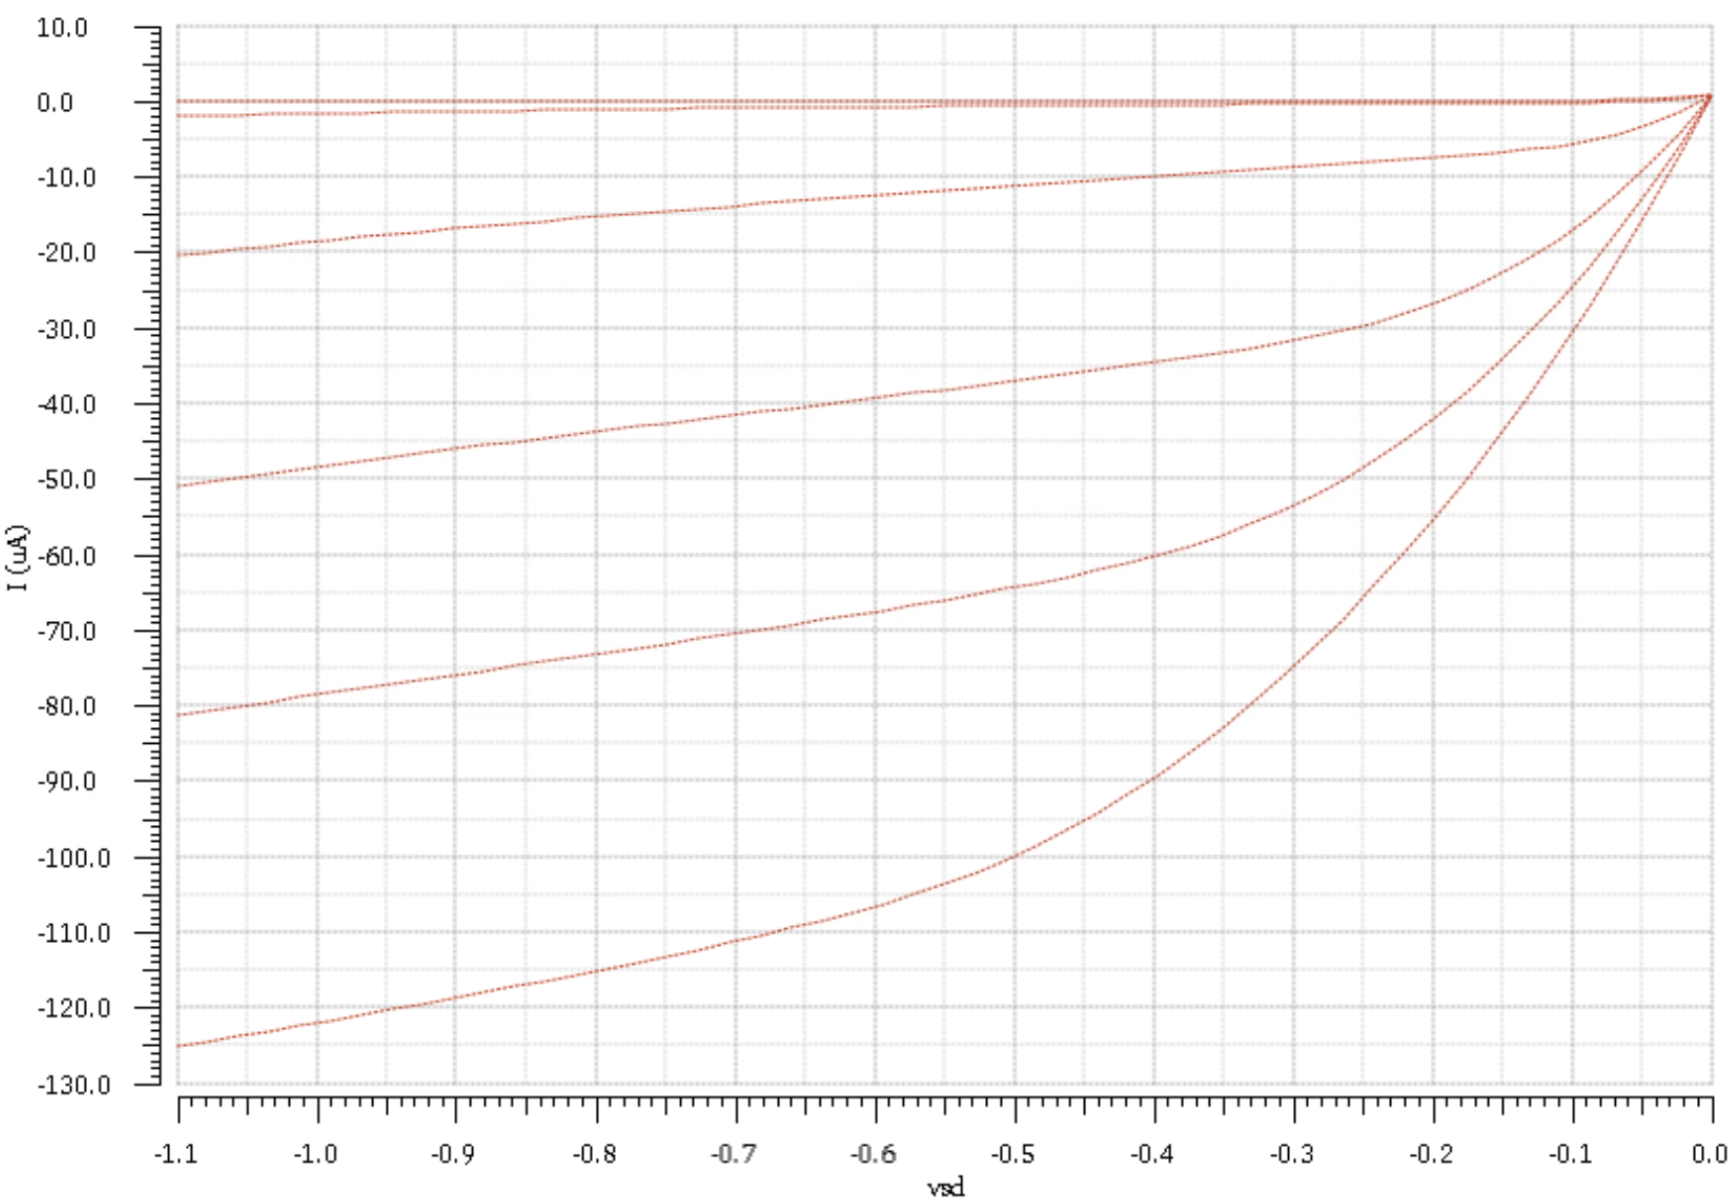
\includegraphics[width = .5\textwidth]{pmos-5.png}}
        
        PMOS: $V_B = -0.5V$
    \end{center}
    \begin{center}
        There are small difference between the curves, the top amplitudes change and in some places it seems like the shape of the curves also change, I think this because the spacing between the curves seem to be different between the figures. From looking at these graphs it seems like the parameter it changes is the voltage threshold, this makes sense on the smaller scale, because the voltage on the base is different, the voltage difference between the gate and the base must be higher or lower to compensate for the base voltage change and to cause the pinch off to occur.
    \end{center}
\end{enumerate}
\end{document}
